\documentclass[../ManualeUtente_v2.0.0.tex]{subfiles}

\begin{document}

	\section{Area dedicata agli ospiti}
	\label{sub:GuestArea}
	L'area dedicata agli ospiti si estende a tutto ciò che permette un'interazione con l'assistente virtuale, esclusa la parte di amministrazione precedentemente descritta.
	Durante la conversazione con Alexa, l'ospite sarà ulteriormente guidato tramite alcune funzionalità visuali, oltre che a quelle vocali, che sono di seguito:

		\begin{itemize}
			\item L'avvio e l'interruzione della sessione;
			% \item La visualizzazione dei suggerimenti;
			% \item La visualizzazione dell'ultima risposta.
		\end{itemize}

		\subsection{Avvio ed interruzione sessione}
		\label{sub:StartStopSession}
		Un ospite che intende iniziare una conversazione con l'assistente virtuale dovrà necessariamente avviarla tramite interazione a schermo con l'icona dedicata.

		Per interrompere \textbf{in modo manuale} una conversazione con l'AV, l'utente non dovrà fare altro che ripetere la stessa operazione.

		La conclusione della sessione con l'assistente virtuale avviene invece \textbf{in modo automatico} in due casi:
		\begin{itemize}
			\item L'ospite ha terminato l'intero \gls{workflow} della conversazione;
			\item Timeout di Alexa per inattività dopo 8 secondi, dopo che quest'ultima ha già ripetuto una seconda volta la domanda.
		\end{itemize}

		Di seguito verranno elencati i vari stati che appariranno all'ospite durante la fase di interazione con \atavi:
		
		\begin{figure}[!h]
			\centering
		 	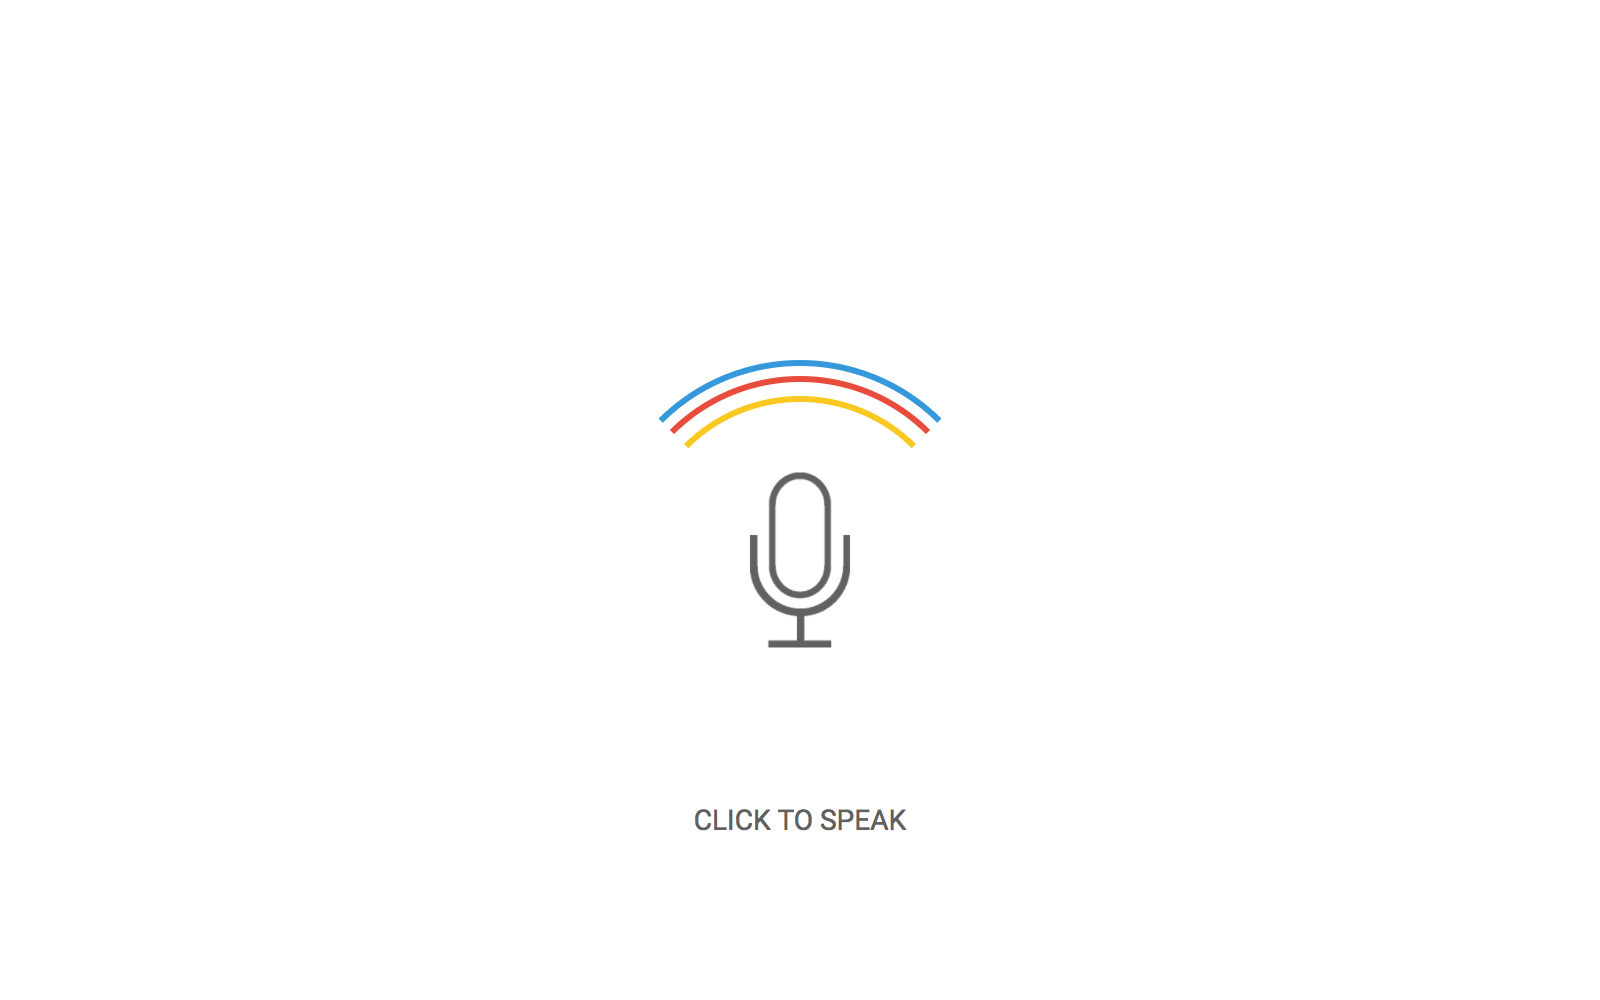
\includegraphics[width=\textwidth]{Screenshot/guest-speak.png}
			\caption{Pagina ospiti - Stato iniziale}
			\label{fig:label}
		\end{figure}
		
		\begin{figure}[!h]
			\centering
		 	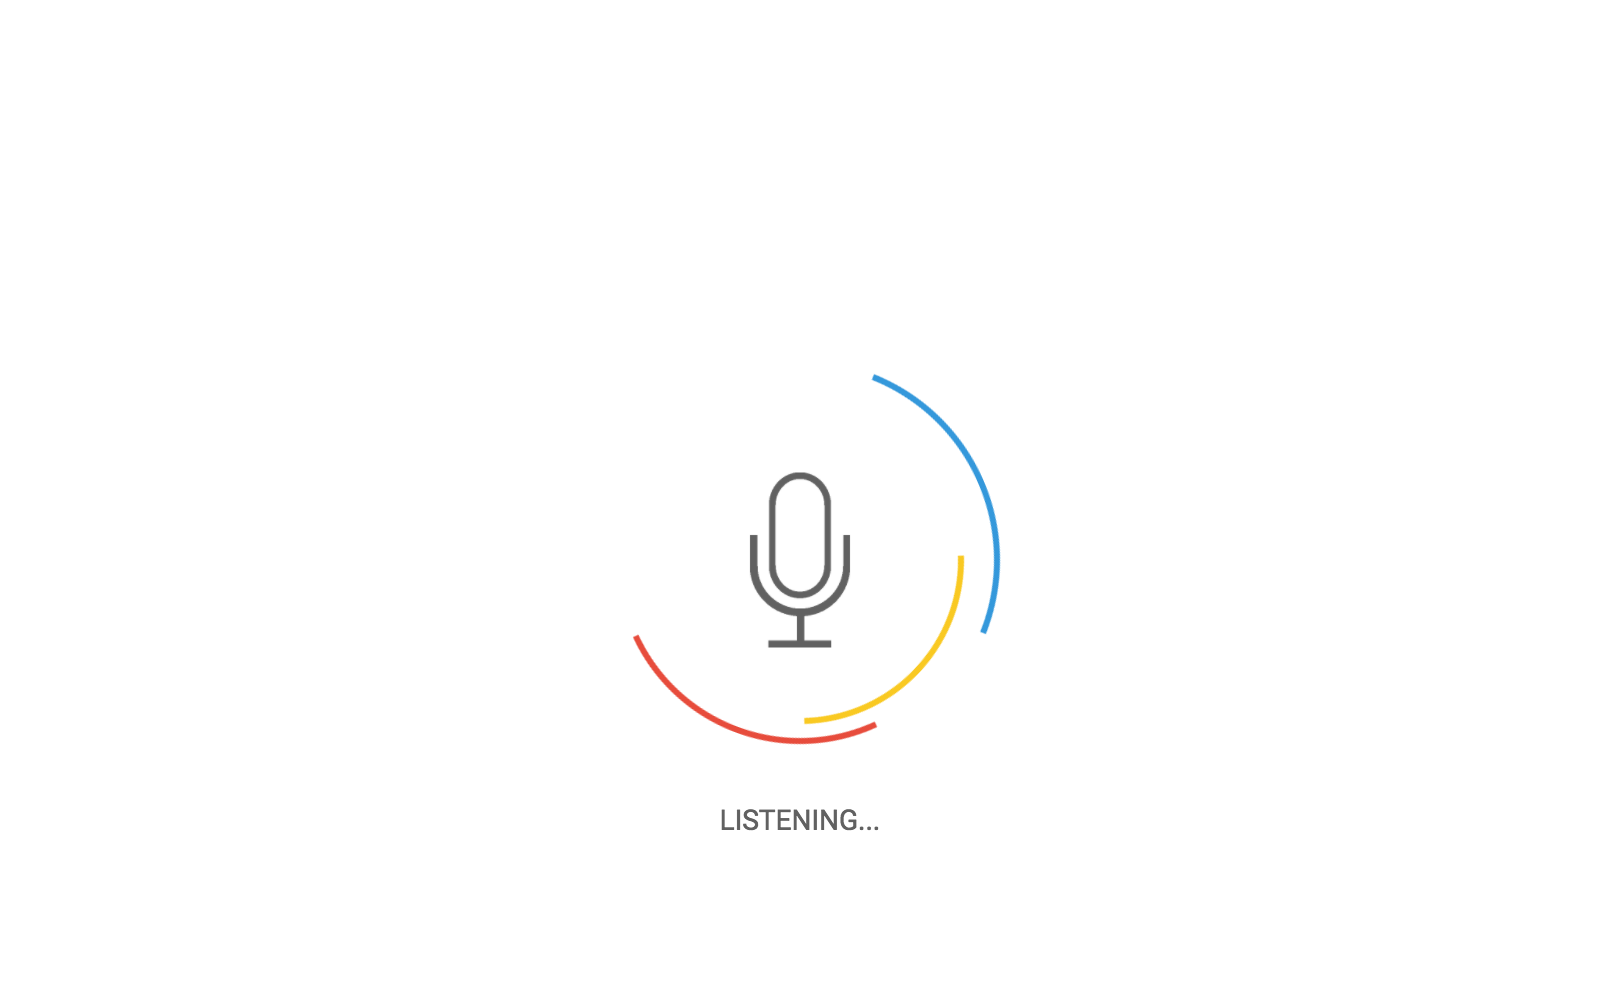
\includegraphics[width=\textwidth]{Screenshot/guest-listening.png}
			\caption{Pagina ospiti - Stato ascolto input vocale}
			\label{fig:label}
		\end{figure}
		
		\begin{figure}[!h]
			\centering
		 	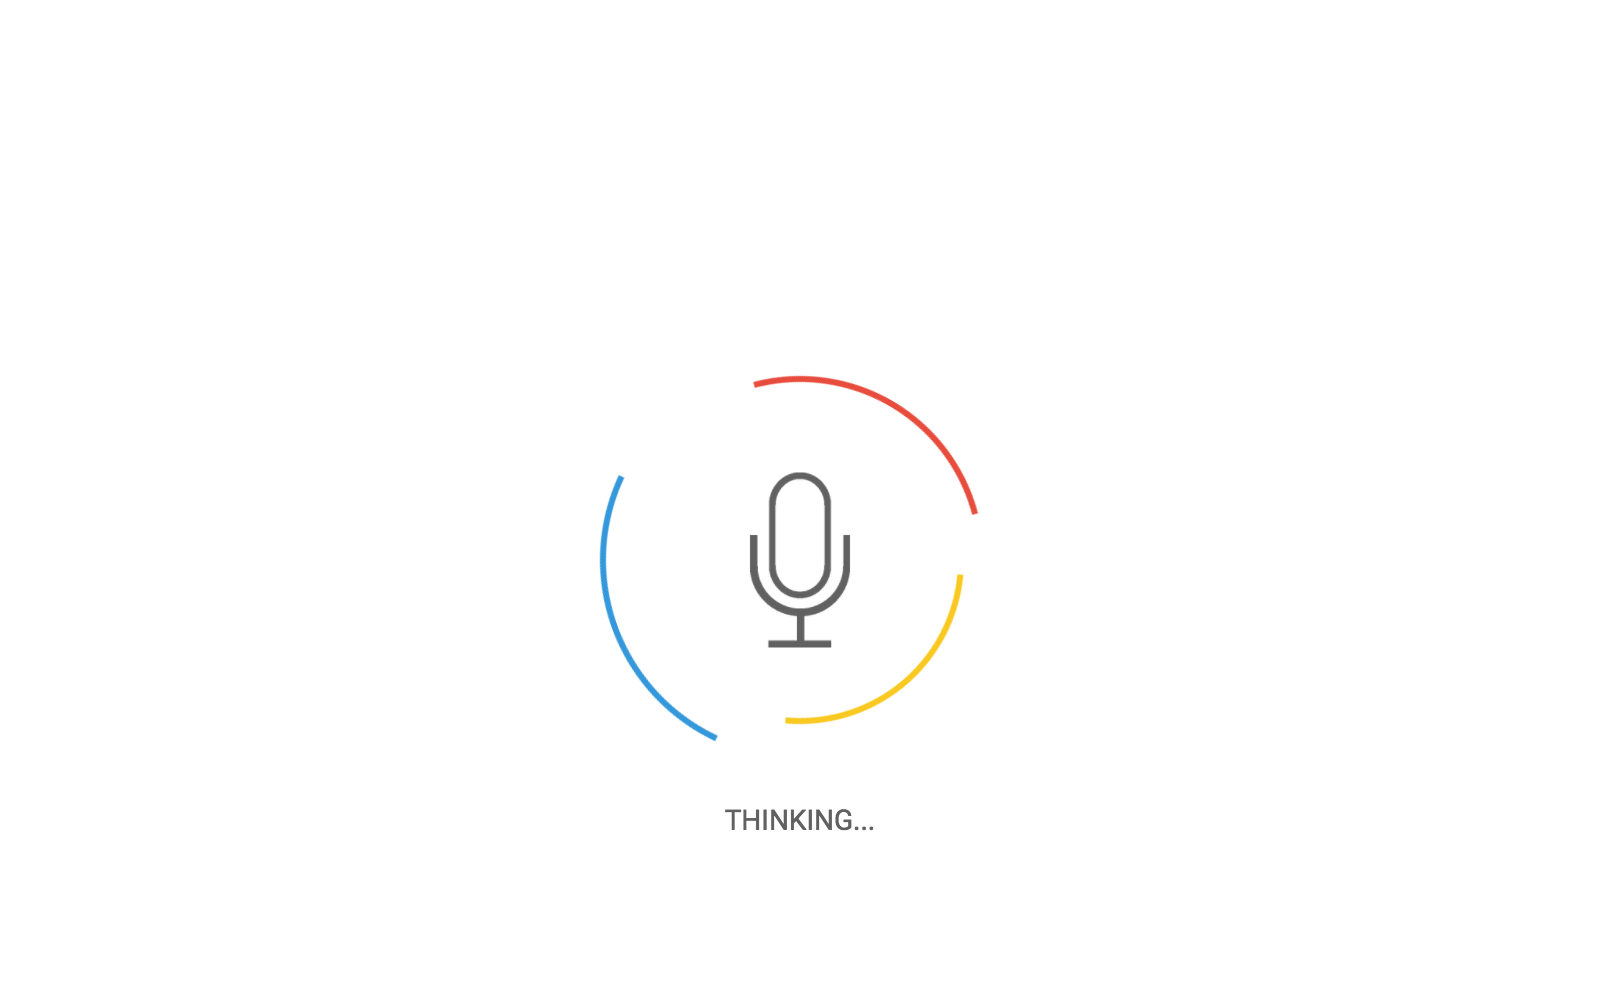
\includegraphics[width=\textwidth]{Screenshot/guest-thinking.png}
			\caption{Pagina ospiti - Stato elaborazione input vocale tramite AVS}
			\label{fig:label}
		\end{figure}

		\begin{figure}[!h]
			\centering
		 	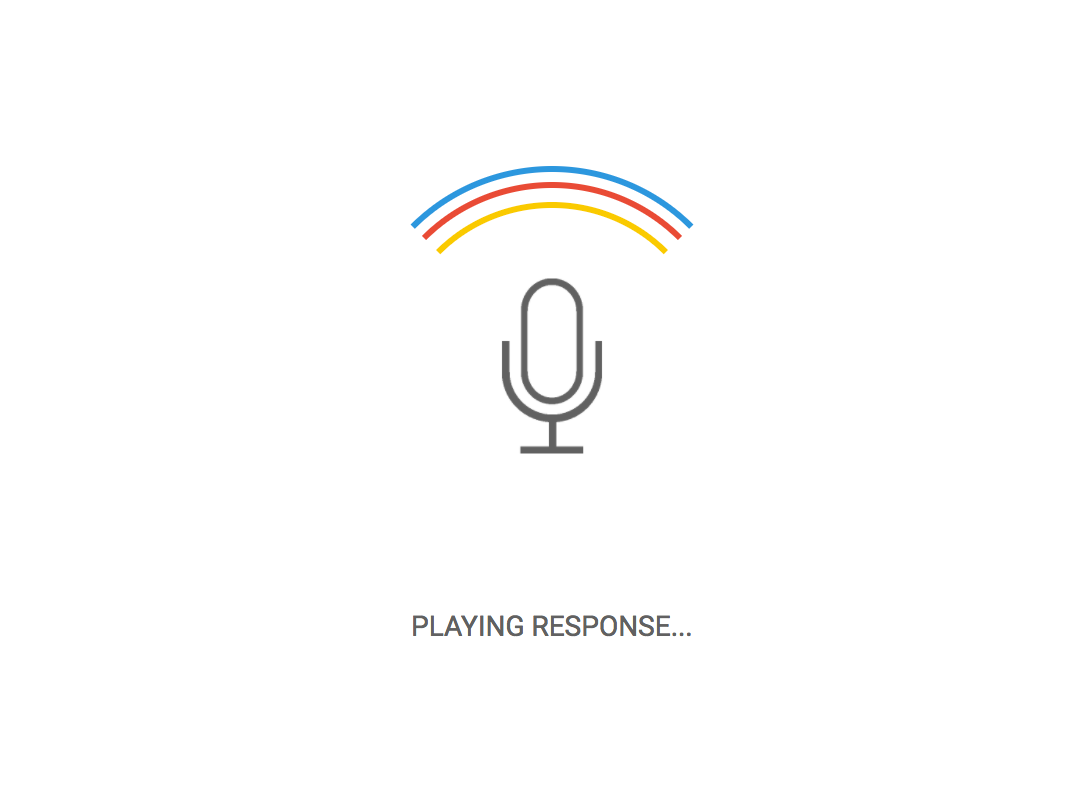
\includegraphics[scale=0.6]{Screenshot/playing-response.png}
			\caption{Pagina ospiti - Riproduzione della risposta da parte di \atavi}
			\label{fig:label}
		\end{figure}

	\begin{comment}
		\subsection{Suggerimenti aziende}
		\label{sub:SuggestionsFirms}
		Il Workflow della conversazione con Alexa prevede che la prima domanda posta ad un ospite sia quella del nome dell'azienda a cui l'ospite appartiene.

		A seguito della risposta dell'ospite, quest'ultimo potrà visualizzare a schermo una lista con i nomi delle aziende che l'assistente virtuale suggerisce dopo aver elaborato l'input ricevuto.

		Aspetto molto importante di questa funzionalità: \textbf{l'ospite potrà interagire a schermo} selezionando la voce che preferisce fra tutte quelle proposte o, nel caso sia corretto il nome compreso dall'AV, continuare la conversazione.
		Viene riportato qui sotto un esempio della schermata visualizzata.

		% \begin{figure}[!h]
		% 	\centering
		% 	\includegraphics[width=\textwidth]{}
		% 	\caption{caption}
		% 	\label{fig:label}
		% \end{figure}

		\subsection{Visualizza ultima risposta}
		\label{sub:lastAnswer}
		Un'altra funzionalità dell'applicazione è quella di offrire un riscontro visivo dell'ultima risposta fornita dall'ospite ad Alexa.
		Questo servizio è fondamentale per migliorare l'esperienza d'utilizzo dell'utente poiché a quest'ultimo viene fornito un feedback dinamico ed immediato di ciò che l'assistente virtuale comprende in seguito alle sue risposte, così da migliorare ed ottimizzare l'intera conversazione ed aiutare l'ospite ad interagire correttamente con Alexa.
		Si riporta un esempio della schermata visualizzata per questa funzionalità.

		% \begin{figure}[!h]
		% 	\centering
		% 	\includegraphics[width=\textwidth]{}
		% 	\caption{caption}
		% 	\label{fig:label}
		% \end{figure}
	\end{comment}

\end{document}
